\chapter{Bord beheren}

\section{Lijst van borden}

In het hoofdscherm \korteverwijzing[fig:overzicht] heb je in het midden van het scherm reeds een overzicht van jouw persoonlijke borden. Om een overzicht te krijgen van alle borden waartoe je toegang hebt maak je gebruik van de knop ``borden''  \korteverwijzing[fig:borden].
\\

\begin{figure}[h]
	\centering
	
\includegraphics[scale=.7]{./afbeeldingen/borden.png}
	\caption{Borden tonen}
	\label{fig:borden}	
\end{figure} 

\noindent
Eens je deze functionalteit geactiveerd hebt krijg je een lijst  \korteverwijzing[fig:lijst_borden] te zien met daarin alle borden waaraan je verbonden bent. Het is eveneens mogelijk om te zoeken naar een specifiek bord in deze lijst. Je kan dan het gewenste bord openen door dit te selecteren.\\

\begin{figure}[H]
	\centering
	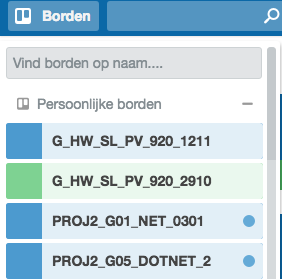
\includegraphics[scale=.5]{./afbeeldingen/lijst_borden.png}
	\caption{Voorbeeldlijst van al jouw borden}
	\label{fig:lijst_borden}	
\end{figure} 

\section{Bord aanmaken}

Een nieuw bord kan op twee manieren aamgemaakt worden:
\begin{enumerate}
	\item 
		\begin{enumerate}
			\item Activeer de ``+'' knop \korteverwijzing[fig:aanmaken_start];
			\item Selecteer nu ``Bord aanmaken'' \korteverwijzing[fig:aanmaken];
			\item Voer een naam in en kies het gewenste team \korteverwijzing[fig:nieuw_bord];
			\item Bevestig de ingevoerde waarden met ``aanmaken'' en het nieuwe Trellobord wordt aangemaakt en onmiddellijk geopend \korteverwijzing[fig:leeg_bord].
		\end{enumerate}
	\item 
		\begin{enumerate}
			\item Activeeer de ``Maak nieuw bord aan ...'' knop \korteverwijzing[fig:nieuw_bord_maken];
			\item Voer een naam in en kies het team \korteverwijzing[fig:nieuw_bord];
			\item Bevestig de ingevoerde waarden met ``aanmaken'' en het nieuwe Trellobord wordt aangemaakt en onmiddellijk geopend \korteverwijzing[fig:leeg_bord].
		\end{enumerate}
\end{enumerate}
\hfil
\begin{figure}[H]
	\centering
	\begin{subfigure}{.5\textwidth}
		\centering
		
\includegraphics[scale=1]{./afbeeldingen/plus.png}
		\captionof{figure}{Aanmaken}
		\label{fig:aanmaken_start}
	\end{subfigure}%
	\begin{subfigure}{.5\textwidth}
		\centering
		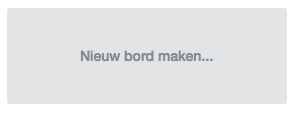
\includegraphics[width=.9\textwidth]{./afbeeldingen/nieuw_bord_maken.png}
		\captionof{figure}{Nieuw bord maken ...}
		\label{fig:nieuw_bord_maken}
	\end{subfigure}\hfill
	\begin{subfigure}{.5\textwidth}
		\centering
		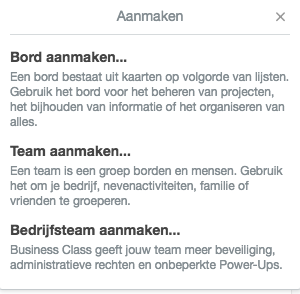
\includegraphics[width=\textwidth]{./afbeeldingen/aanmaken.png}
		\captionof{figure}{Aanmaken}
		\label{fig:aanmaken}
	\end{subfigure}%
	\begin{subfigure}{.5\textwidth}
		\centering
		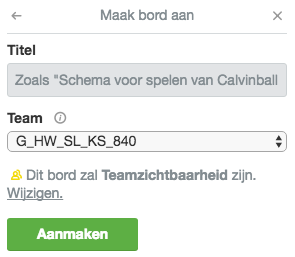
\includegraphics[width=\textwidth]{./afbeeldingen/nieuw_bord.png}
		\captionof{figure}{Nieuw bord}
		\label{fig:nieuw_bord}
	\end{subfigure}
	\caption{Aanmaken van een nieuw Trellobord}
	\label{fig:aanmaken_bord}
\end{figure}

\begin{figure}[H]
	\centering
	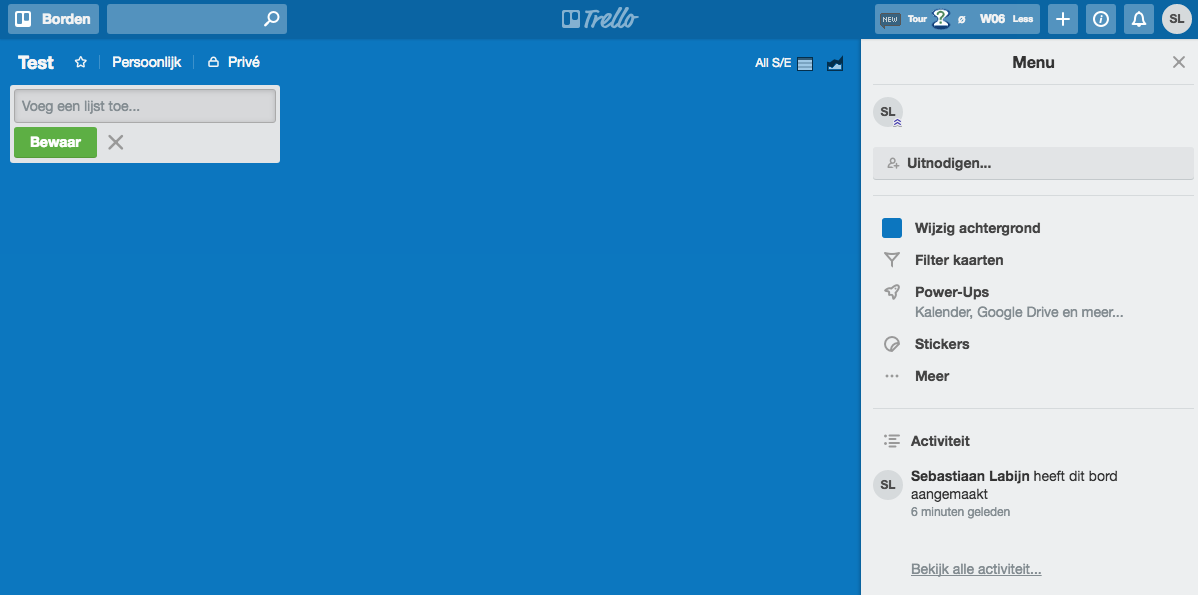
\includegraphics[width=\textwidth]{./afbeeldingen/leeg_bord.png}
	\caption{Een nieuw aangemaakt bord}
	\label{fig:leeg_bord}	
\end{figure} 

\section{Bord wijzigen}

Onderstaande lijst toont een overzicht met functionaliteiten \korteverwijzing[fig:leeg_bord_genummerd] om het bord te wijzigen die overeenstemmen met een nummer op die figuur. Deze worden uitgebreid beschreven in de volgende paragrafen.

\begin{enumerate}[nolistsep]
	\item Naam wijzigen;
	\item Team wijzigen;
	\item Zichtbaarheid aanpassen;
	\item Lijsten wijzigen \verwijzing[chapter:lijsten_beheren];
	\item Kaarten wijzigen \verwijzing[chapter:kaarten_beheren];
	\item Leden wijzigen  \verwijzing[chapter:leden_beheren];
	\item Weergave Trellobord aanpassen.
\end{enumerate}

\paragraaf{Naam wijzigen}
\noindent
\\Om de naam van het Trellobord te wijzigen onderneem je volgende stappen:
\begin{enumerate}[nolistsep]
	\item Selecteer de huidige naam;
	\item Voer de nieuwe naam in;
	\item Bevestig de wijziging.
\end{enumerate}	

\paragraaf{Team wijzigen}
\noindent
\\Selecteer het huidige team en kies daarna de gewenste waarde. Indien er nog geen team aan het bord gekoppeld is zie je de waarde ``Persoonlijk". Wanneer je een team kiest kan je extra opties voor dat team instellen \korteverwijzing[fig:wijzig_Team]. Als het team nog niet bestaat kan je via dit scherm ook de functionaliteit starten om het aan te maken \verwijzing[chapter:team_beheren].

\begin{figure}[H]
	\centering
	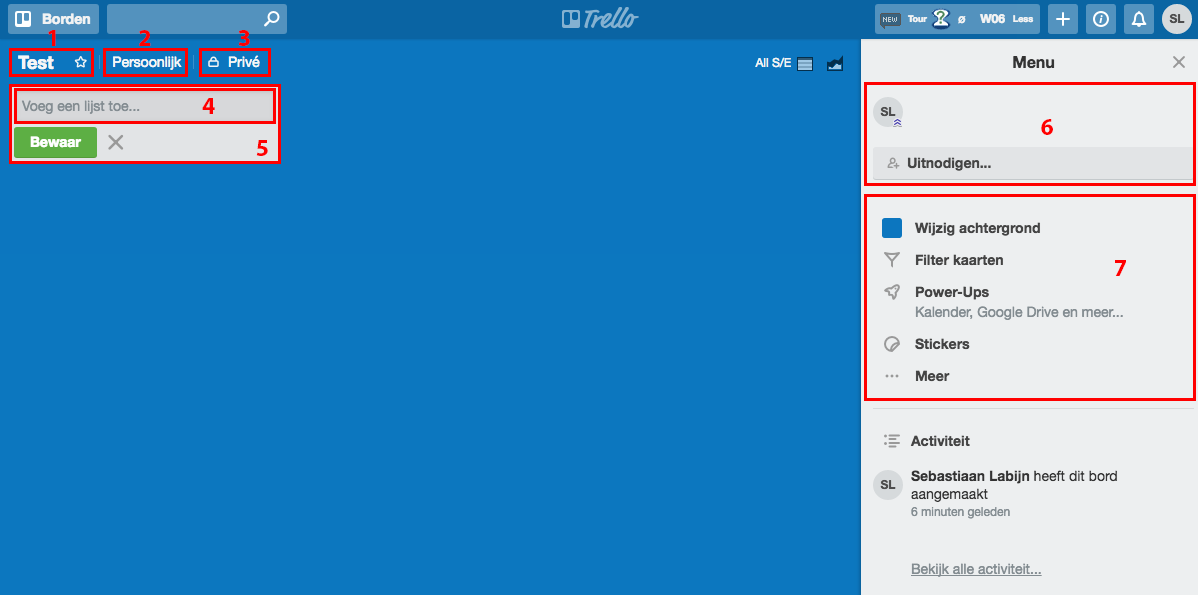
\includegraphics[width=\textwidth]{./afbeeldingen/leeg_bord_genummerd.png}
	\caption{Aanduiding belangrijkste functionaliteiten op een bord}
	\label{fig:leeg_bord_genummerd}	
\end{figure} 

\begin{figure}[H]
	\centering
	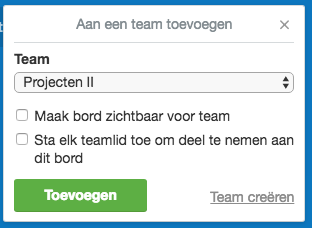
\includegraphics[scale=0.5]{./afbeeldingen/wijzig_team.png}
	\caption{Team wijzigen}
	\label{fig:wijzig_Team}	
\end{figure} 

\paragraaf{Zichtbaarheid aanpassen}
\noindent
\\Selecteer de huidige zichtbaarheid en kies daarna de gewenste zichtbaarheid. In Trello is er keuze uit drie verschillende modi:
\begin{itemize}
	\item Priv\'e: Enkel zichtbaar voor jou en de toegevoegde leden;
	\item Team: Enkel zichtbaar voor jou en de teamleden;
	\item Openbaar:  Zichtbaar voor iedereen die over de hyperlink naar het bord beschikt.
\end{itemize}	

\pagebreak

\paragraaf{Weergave bord aanpassen}
\noindent
\\Er is de mogelijkheid om onder andere volgende eigenschappen van het Trellobord aan te passen:
\begin{itemize}
	\item Achtergrond: Kies een achtergrondkleur of laad een foto op als achtergrond;
	\item Filter kaarten: Toon enkel kaarten die aan de filter voldoen;
	\item Power-ups: Integreer jouw Trellobord met tal van andere toepassingen (b.v.: Slack\footnote{\url{http://www.slack.com}}, GitHub\footnote{\url{http://www.github.com}});
	\item Stickers: Gebruik stickers.
\end{itemize}